\chapter{ИССЛЕДОВАНИЕ АЛГОРИТМА ПЛАНИРОВАНИЯ ТРАЕКТОРИЙ С ЗАДАННОЙ ГЛАДКОСТЬЮ}

\section{Цель работы}

Исследование алгоритма планирования траекторий с заданной гладкостью.

\section{Задание}

\begin{enumerate}
\item Сформировать бинарную карту размером 10 на 10 ячеек. На карте не менее трети ячеек должны быть недоступными к посещению. Выбрать начальную и конечную точки так, чтобы траектория между ними содержала не менее 10 ячеек и не менее трех поворотов. Применить алгоритм А* для нахождения пути от начальной точки к конечной.

\item Сгенерировать C$^0$-гладкую траекторию через полученные точки. Декартовы координаты точек принять равными номеру ячейки карты по горизонтали и вертикали соответственно.

\item Сгенерировать C$^1$-гладкую траекторию для тех же точек.

\item Сгенерировать C$^2$-гладкую траекторию для тех же точек.

\item Осуществить сглаживание траектории, полученной в пункте 2 при помощи В-сплайна.
\end{enumerate}

\section{Описание алгоритмов планирования траектории}

\subsection{Алгоритм A*}

Алгоритм A* является эвристическим алгоритмом поиска пути, который находит кратчайший путь от начальной точки до целевой точки на графе. Алгоритм использует функцию оценки $f(n) = g(n) + h(n)$, где:
\begin{itemize}
\item $g(n)$ --- стоимость пути от начальной точки до узла $n$
\item $h(n)$ --- эвристическая оценка стоимости пути от узла $n$ до целевой точки
\end{itemize}

В данной работе используется манхэттенское расстояние в качестве эвристической функции:
$$h(n) = |x_n - x_{goal}| + |y_n - y_{goal}|$$

Алгоритм A* гарантирует нахождение оптимального пути при условии, что эвристическая функция не переоценивает реальную стоимость.

\textbf{Реализация алгоритма A*:} Для выполнения первого пункта задания была создана бинарная карта размером 10×10 ячеек. Процесс создания включал следующие этапы:

\begin{enumerate}
\item \textbf{Инициализация сетки:} Создана матрица размером 10×10, заполненная нулями (свободные ячейки).
\item \textbf{Размещение препятствий:} Случайным образом размещены препятствия (значение 1) в 35\% ячеек (35 из 100), что превышает требуемые 33\%.
\item \textbf{Воспроизводимость:} Использован фиксированный seed (42) для обеспечения воспроизводимости результатов.
\end{enumerate}

Для выбора подходящих начальной и конечной точек был реализован алгоритм поиска, который проверяет доступность точек (не являются препятствиями), находит путь между точками с помощью алгоритма A*, проверяет, что длина пути составляет не менее 10 ячеек, и подсчитывает количество поворотов (должно быть не менее 3).

Алгоритм A* реализован с использованием 8-связности (диагональные перемещения разрешены). Основные компоненты включают открытый список (приоритетная очередь для хранения узлов, которые нужно исследовать), закрытый список (множество уже исследованных узлов), эвристическую функцию (манхэттенское расстояние) и восстановление пути (обратный проход от конечной точки к начальной).

\textbf{Результат выполнения:} Найдены начальная точка (2, 0) и конечная точка (4, 9) с путем длиной 10 ячеек и 7 поворотами, что удовлетворяет всем требованиям задания.

\subsection{Генерация C$^0$-гладкой траектории}

C$^0$-гладкость означает непрерывность функции без разрывов. Для генерации C$^0$-гладкой траектории используется кусочно-линейная интерполяция между точками пути, найденного алгоритмом A*. Координаты точек траектории вычисляются как:

$$x(t) = \text{interp1}(t, x_{path}, \text{kind='linear'})$$
$$y(t) = \text{interp1}(t, y_{path}, \text{kind='linear'})$$

где $t \in [0, 1]$ --- параметр траектории.

\textbf{Процесс генерации C$^0$-гладкой траектории:} Точки пути, полученные алгоритмом A*, представлены в виде индексов ячеек (строка, столбец). Для создания траектории координаты преобразуются следующим образом: $x$-координата = номер столбца ячейки, $y$-координата = номер строки ячейки. Создается параметр $t \in [0, 1]$, где $t = 0$ соответствует начальной точке, $t = 1$ соответствует конечной точке, а промежуточные значения равномерно распределены между точками пути. Используется функция \texttt{interp1d} из библиотеки SciPy с параметром \texttt{kind='linear'} для создания кусочно-линейной траектории между точками пути.

\textbf{Результат:} Создана C$^0$-гладкая траектория, которая проходит точно через все точки пути A*, но имеет резкие углы в точках поворота.

\subsection{Генерация C$^1$-гладкой траектории}

C$^1$-гладкость означает непрерывность первой производной функции. Для генерации C$^1$-гладкой траектории используется кубическая сплайн-интерполяция с естественными граничными условиями:

$$x(t) = \text{CubicSpline}(t, x_{path}, \text{bc\_type='natural'})$$
$$y(t) = \text{CubicSpline}(t, y_{path}, \text{bc\_type='natural'})$$

\textbf{Процесс генерации C$^1$-гладкой траектории:} Для обеспечения непрерывности первой производной используется кубическая сплайн-интерполяция с естественными граничными условиями (\texttt{bc\_type='natural'}). Естественные граничные условия означают, что вторые производные на концах траектории равны нулю:
$$\frac{d^2x}{dt^2}\bigg|_{t=0} = \frac{d^2x}{dt^2}\bigg|_{t=1} = 0$$
$$\frac{d^2y}{dt^2}\bigg|_{t=0} = \frac{d^2y}{dt^2}\bigg|_{t=1} = 0$$

\textbf{Результат:} Создана C$^1$-гладкая траектория с непрерывной первой производной, что обеспечивает плавные переходы между сегментами.

\subsection{Генерация C$^2$-гладкой траектории}

C$^2$-гладкость означает непрерывность второй производной функции. Для генерации C$^2$-гладкой траектории используется кубическая сплайн-интерполяция с закрепленными граничными условиями:

$$x(t) = \text{CubicSpline}(t, x_{path}, \text{bc\_type='clamped'})$$
$$y(t) = \text{CubicSpline}(t, y_{path}, \text{bc\_type='clamped'})$$

\textbf{Процесс генерации C$^2$-гладкой траектории:} Для обеспечения непрерывности второй производной используются закрепленные граничные условия (\texttt{bc\_type='clamped'}), которые фиксируют значения первых производных на концах. Граничные производные вычисляются как:
$$\frac{dx}{dt}\bigg|_{t=0} = \frac{x_1 - x_0}{t_1 - t_0}, \quad \frac{dx}{dt}\bigg|_{t=1} = \frac{x_n - x_{n-1}}{t_n - t_{n-1}}$$

\textbf{Результат:} Создана C$^2$-гладкая траектория с непрерывными первой и второй производными, обеспечивающая максимальную гладкость.

\subsection{B-сплайн сглаживание}

B-сплайн сглаживание используется для получения более гладкой траектории. В данной работе применяется UnivariateSpline с кубическими B-сплайнами:

$$x(t) = \text{UnivariateSpline}(t, x_{path}, \text{k=3})$$
$$y(t) = \text{UnivariateSpline}(t, y_{path}, \text{k=3})$$

\textbf{Процесс B-сплайн сглаживания:} Используется \texttt{UnivariateSpline} с кубическими B-сплайнами (степень k=3) для сглаживания C$^0$-гладкой траектории. B-сплайн автоматически подбирает параметр сглаживания s для минимизации ошибки аппроксимации при сохранении гладкости.

\textbf{Результат:} Получена наиболее гладкая траектория с минимальными значениями кривизны.

\section{Вычисление кривизны траекторий}

Кривизна траектории вычисляется по формуле:

$$\kappa(t) = \frac{|x'(t)y''(t) - y'(t)x''(t)|}{(x'(t)^2 + y'(t)^2)^{3/2}}$$

где $x'(t)$, $y'(t)$ --- первые производные, $x''(t)$, $y''(t)$ --- вторые производные по параметру $t$.

\textbf{Метод вычисления:} Для вычисления кривизны используются численные производные, полученные с помощью функции \texttt{np.gradient} из библиотеки NumPy. Первые производные вычисляются как $dx/dt = \text{gradient}(x, t)$ и $dy/dt = \text{gradient}(y, t)$, а вторые производные как $d^2x/dt^2 = \text{gradient}(dx/dt, t)$ и $d^2y/dt^2 = \text{gradient}(dy/dt, t)$. Для избежания деления на ноль используется функция \texttt{np.divide} с параметром \texttt{where}.

\section{Результаты моделирования}

\subsection{Бинарная карта и путь A*}

На рисунке \ref{fig:astar_path} представлена бинарная карта размером 10×10 ячеек с препятствиями (черные ячейки) и путь, найденный алгоритмом A*. Начальная точка отмечена зеленым квадратом, конечная --- синей звездочкой. Путь показан красной линией.

\begin{figure}[H]
\centering
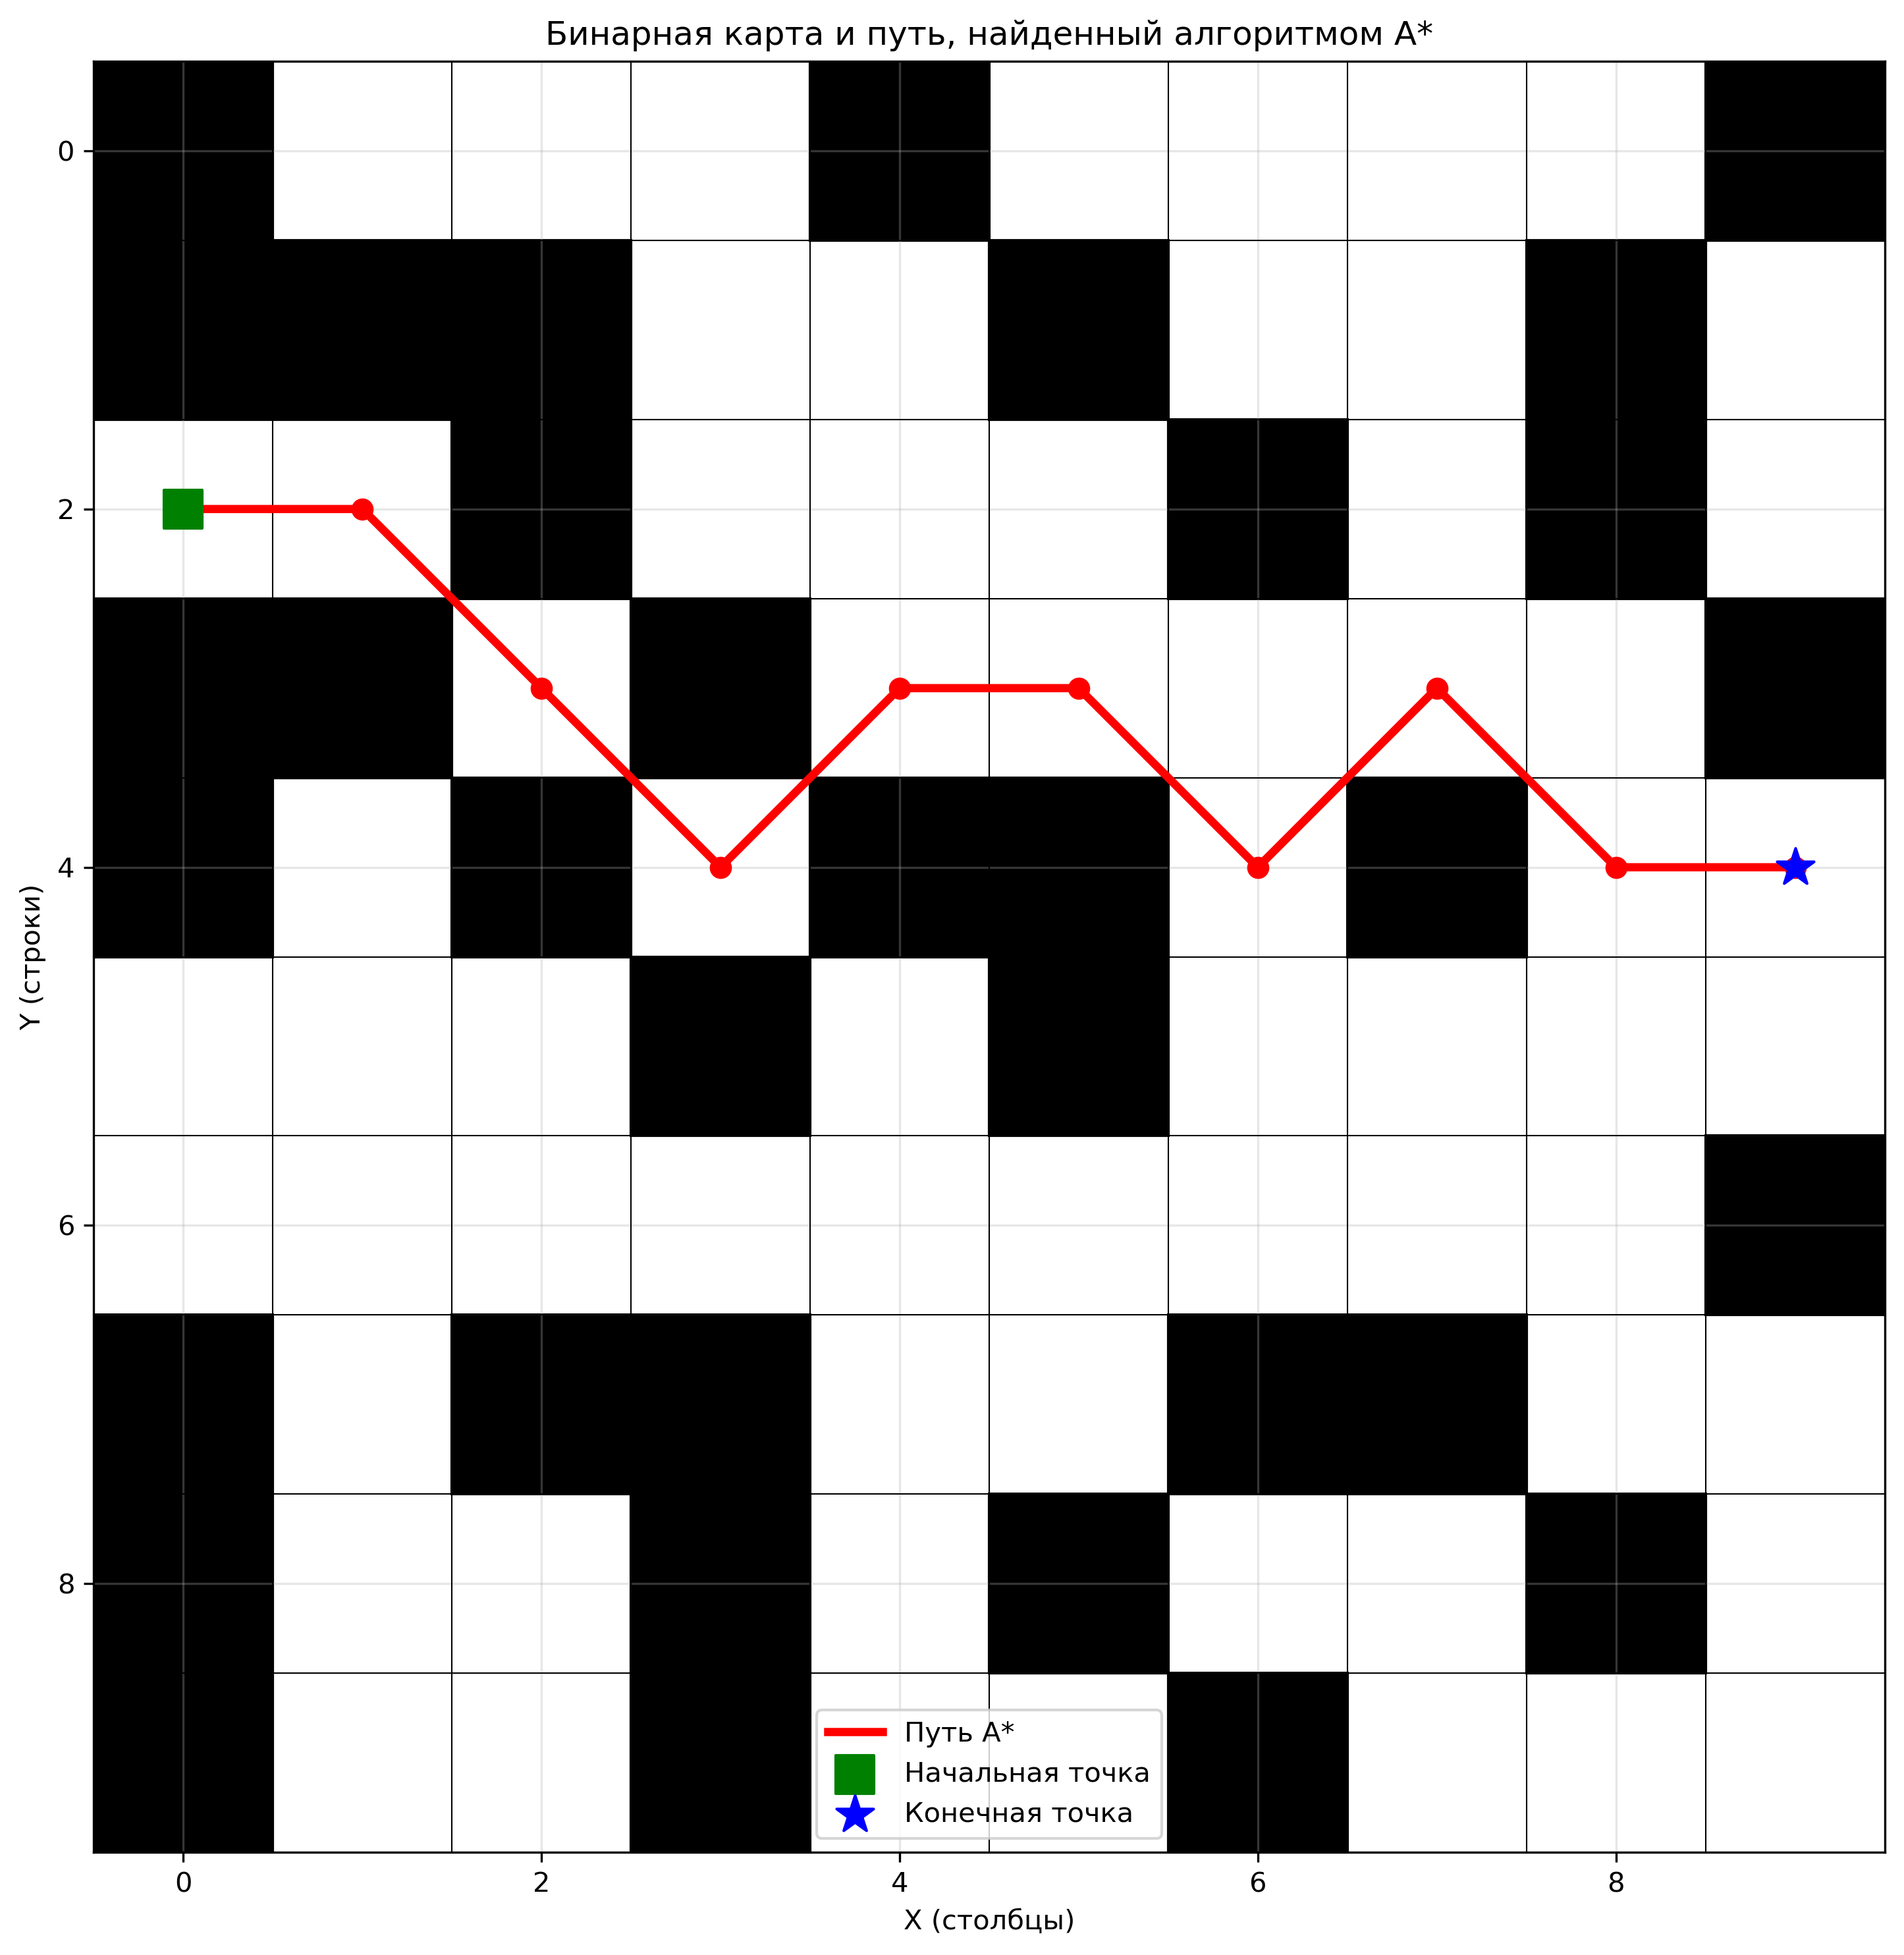
\includegraphics[width=0.8\textwidth]{task1/astar_path.png}
\caption{Бинарная карта и путь, найденный алгоритмом A*}
\label{fig:astar_path}
\end{figure}

Параметры найденного пути:
\begin{itemize}
\item Длина пути: 10 ячеек
\item Количество поворотов: 7
\item Начальная точка: (2, 0)
\item Конечная точка: (4, 9)
\end{itemize}

\subsection{Сравнение траекторий с разной гладкостью}

На рисунке \ref{fig:trajectories_comparison} представлено сравнение всех сгенерированных траекторий.

\begin{figure}[H]
\centering
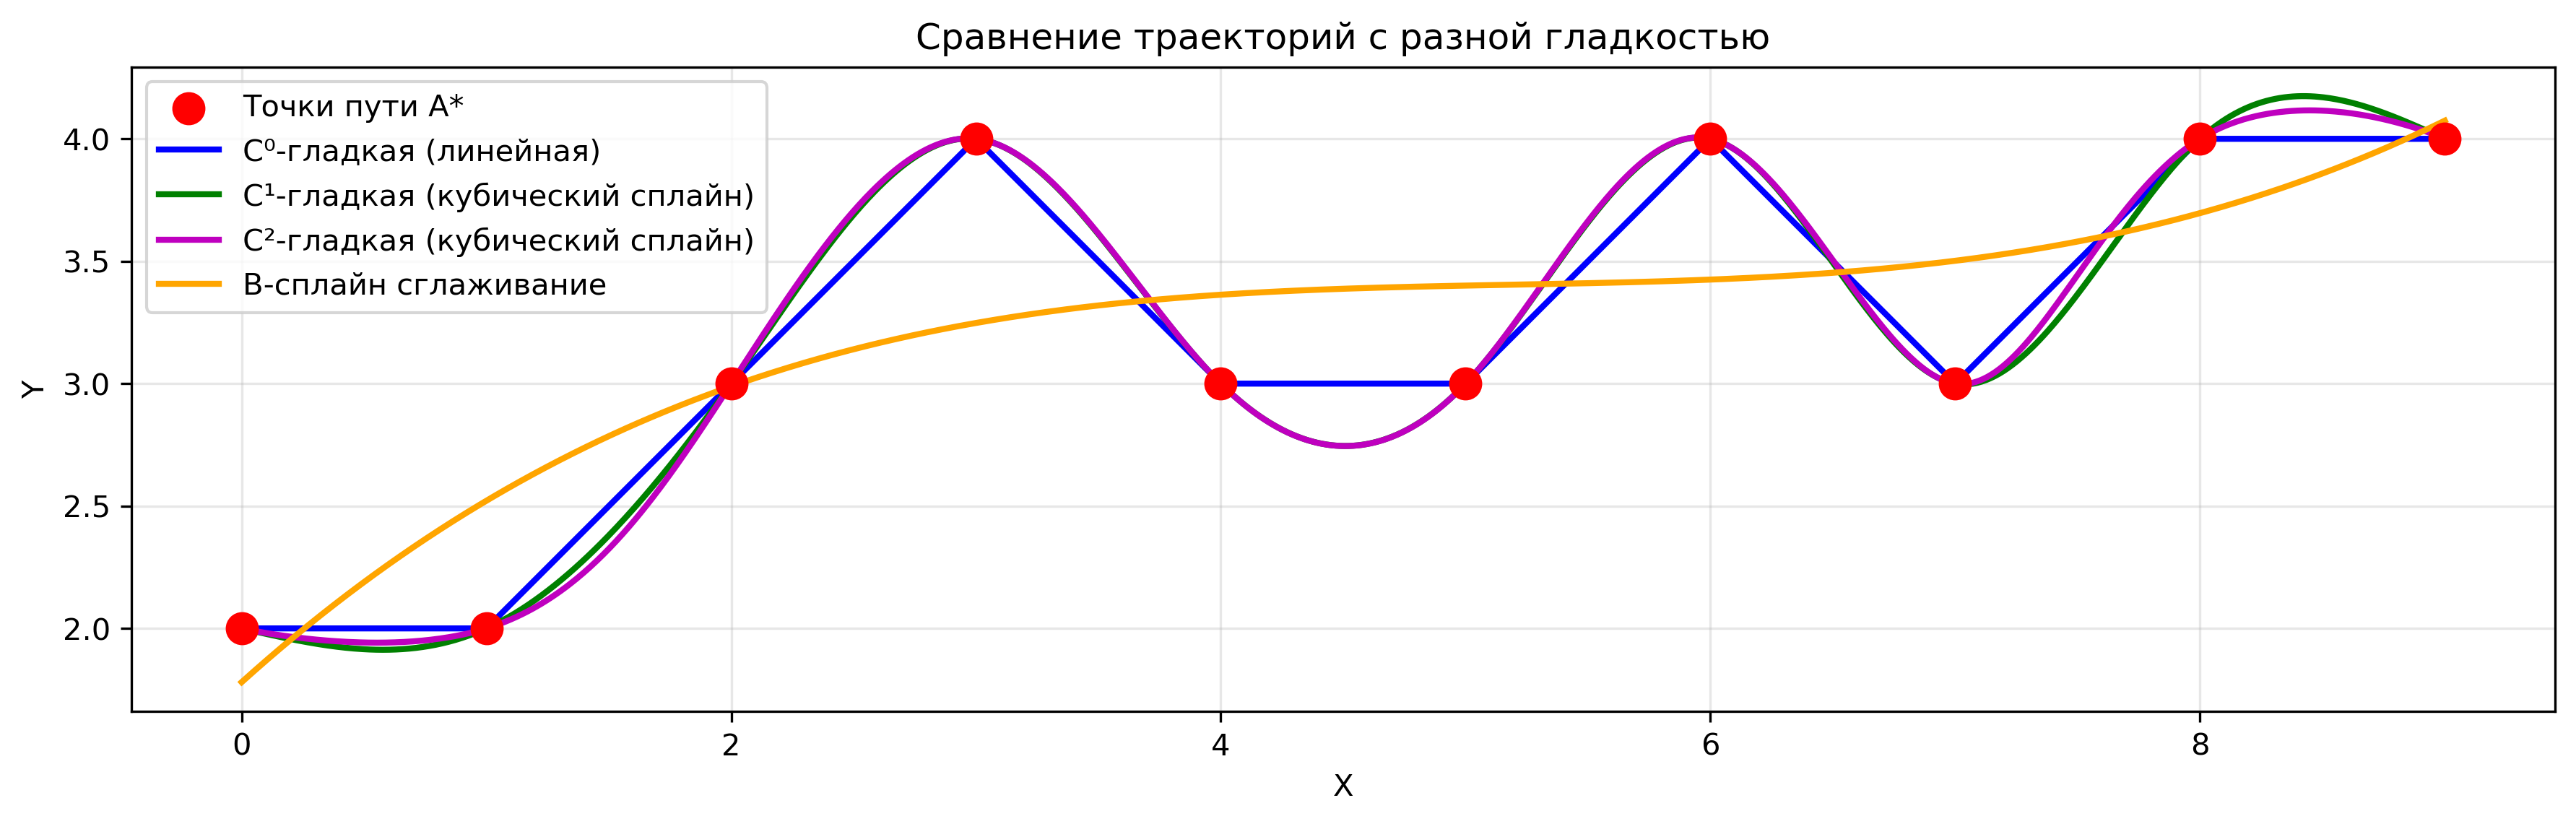
\includegraphics[width=0.9\textwidth]{task2/trajectories_comparison.png}
\caption{Сравнение траекторий с разной гладкостью}
\label{fig:trajectories_comparison}
\end{figure}

\subsection{Анализ кривизн траекторий}

На рисунке \ref{fig:curvature_comparison} представлено сравнение кривизн всех траекторий.

\begin{figure}[H]
\centering
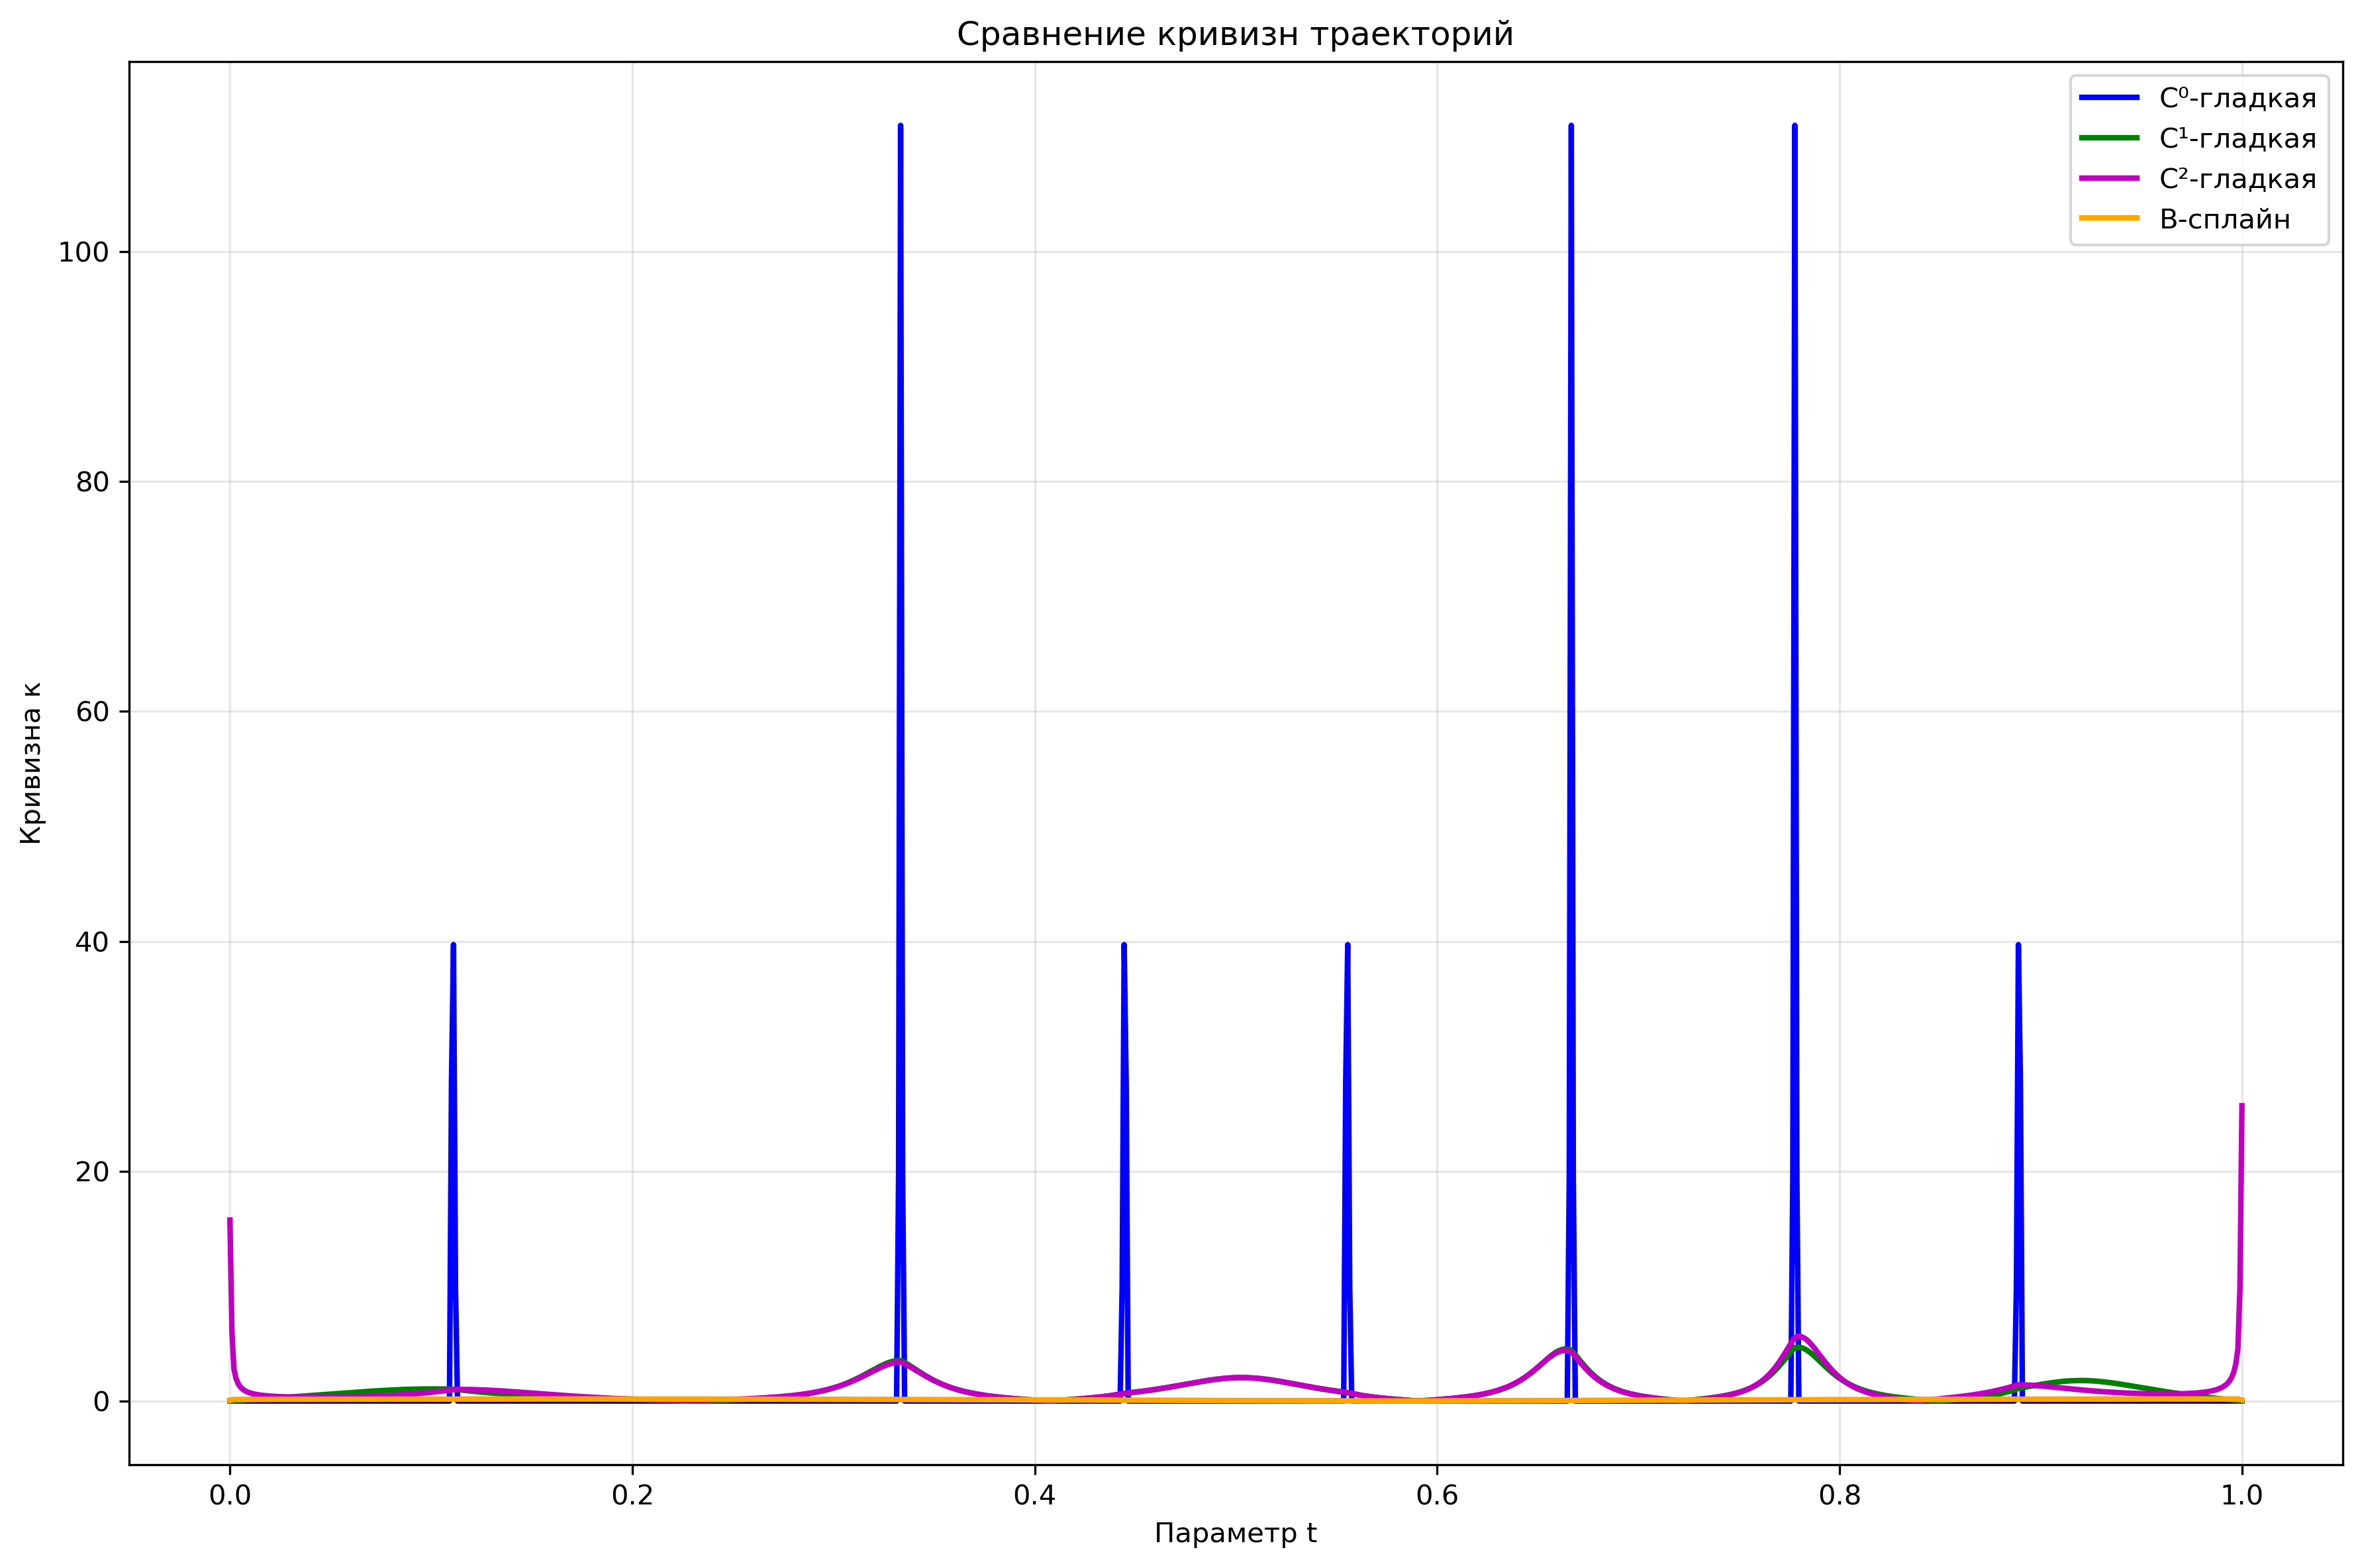
\includegraphics[width=0.9\textwidth]{task2/curvature_comparison.png}
\caption{Сравнение кривизн траекторий}
\label{fig:curvature_comparison}
\end{figure}

Статистика кривизн:
\begin{itemize}
\item C$^0$-гладкая: средняя = 0.7598, максимальная = 111.0000
\item C$^1$-гладкая: средняя = 0.9710, максимальная = 4.6861
\item C$^2$-гладкая: средняя = 1.0420, максимальная = 25.6972
\item B-сплайн: средняя = 0.1189, максимальная = 0.1800
\end{itemize}

\section{Выводы}

Алгоритм A* успешно нашел путь длиной 10 ячеек с 7 поворотами, что удовлетворяет требованиям задания. C$^0$-гладкая траектория имеет наибольшую максимальную кривизну (111.0) из-за резких углов в точках поворота, что делает её непригодной для практического использования. C$^1$-гладкая траектория показывает значительное улучшение по сравнению с C$^0$-гладкой, максимальная кривизна снизилась до 4.69. C$^2$-гладкая траектория имеет промежуточные характеристики между C$^1$-гладкой и B-сплайном. B-сплайн сглаживание обеспечивает наилучшие характеристики с точки зрения гладкости: минимальная средняя кривизна (0.119) и максимальная кривизна (0.18), что делает эту траекторию наиболее подходящей для практического применения. Все траектории с гладкостью выше C$^0$ показывают значительное улучшение характеристик по сравнению с кусочно-линейной траекторией.

